% AUTO-GENERATED by code/ch11_figs.py
\nElevenFit{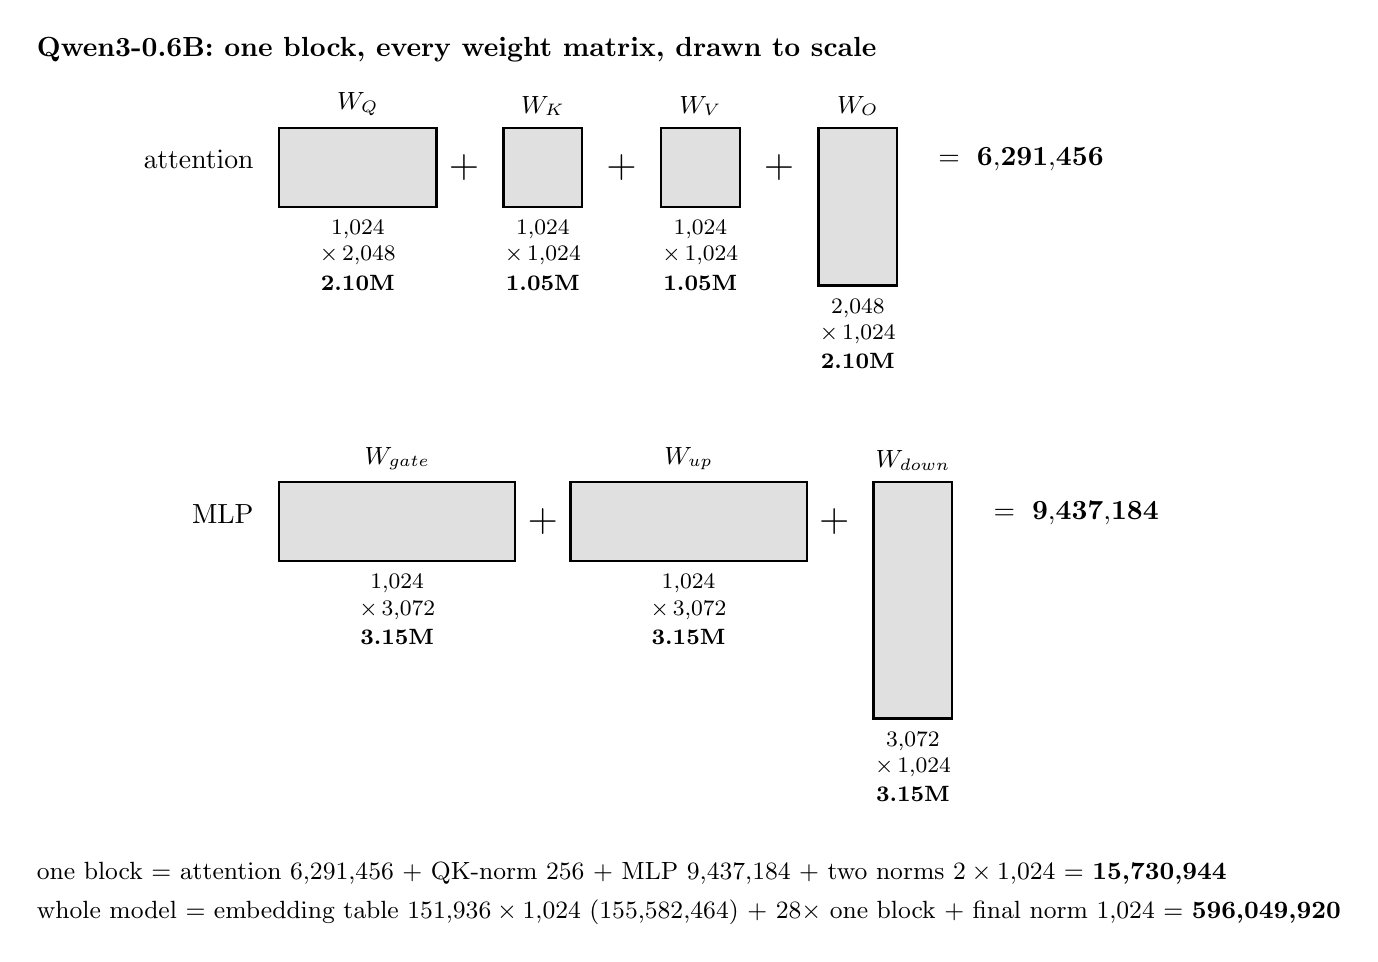
\begin{tikzpicture}
\node[anchor=west, font=\normalsize\bfseries] at (-3.2,1.0) {Qwen3-0.6B: one block, every weight matrix, drawn to scale};
\node[anchor=east, font=\normalsize, align=right] at (-0.200,-0.400) {attention};
\draw[line width=0.8pt, fill=black!12] (0.000,0.000) rectangle (2.000,-1.000);
\node[anchor=south, font=\small] at (1.000,0.030) {$W_Q$};
\node[anchor=north, font=\footnotesize, align=center] at (1.000,-1.050) {1{,}024\\$\times$\,2{,}048\\[1pt]\textbf{2.10M}};
\node[font=\Large] at (2.350,-0.500) {$+$};
\draw[line width=0.8pt, fill=black!12] (2.850,0.000) rectangle (3.850,-1.000);
\node[anchor=south, font=\small] at (3.350,0.030) {$W_K$};
\node[anchor=north, font=\footnotesize, align=center] at (3.350,-1.050) {1{,}024\\$\times$\,1{,}024\\[1pt]\textbf{1.05M}};
\node[font=\Large] at (4.350,-0.500) {$+$};
\draw[line width=0.8pt, fill=black!12] (4.850,0.000) rectangle (5.850,-1.000);
\node[anchor=south, font=\small] at (5.350,0.030) {$W_V$};
\node[anchor=north, font=\footnotesize, align=center] at (5.350,-1.050) {1{,}024\\$\times$\,1{,}024\\[1pt]\textbf{1.05M}};
\node[font=\Large] at (6.350,-0.500) {$+$};
\draw[line width=0.8pt, fill=black!12] (6.850,0.000) rectangle (7.850,-2.000);
\node[anchor=south, font=\small] at (7.350,0.030) {$W_O$};
\node[anchor=north, font=\footnotesize, align=center] at (7.350,-2.050) {2{,}048\\$\times$\,1{,}024\\[1pt]\textbf{2.10M}};
\node[anchor=west, font=\normalsize] at (8.250,-0.400) {$=\ \mathbf{6{,}291{,}456}$};
\node[anchor=east, font=\normalsize, align=right] at (-0.200,-4.900) {MLP};
\draw[line width=0.8pt, fill=black!12] (0.000,-4.500) rectangle (3.000,-5.500);
\node[anchor=south, font=\small] at (1.500,-4.470) {$W_{\text{gate}}$};
\node[anchor=north, font=\footnotesize, align=center] at (1.500,-5.550) {1{,}024\\$\times$\,3{,}072\\[1pt]\textbf{3.15M}};
\node[font=\Large] at (3.350,-5.000) {$+$};
\draw[line width=0.8pt, fill=black!12] (3.700,-4.500) rectangle (6.700,-5.500);
\node[anchor=south, font=\small] at (5.200,-4.470) {$W_{\text{up}}$};
\node[anchor=north, font=\footnotesize, align=center] at (5.200,-5.550) {1{,}024\\$\times$\,3{,}072\\[1pt]\textbf{3.15M}};
\node[font=\Large] at (7.050,-5.000) {$+$};
\draw[line width=0.8pt, fill=black!12] (7.550,-4.500) rectangle (8.550,-7.500);
\node[anchor=south, font=\small] at (8.050,-4.470) {$W_{\text{down}}$};
\node[anchor=north, font=\footnotesize, align=center] at (8.050,-7.550) {3{,}072\\$\times$\,1{,}024\\[1pt]\textbf{3.15M}};
\node[anchor=west, font=\normalsize] at (8.950,-4.900) {$=\ \mathbf{9{,}437{,}184}$};
\node[anchor=north west, font=\small, align=left] at (-3.2,-9.200) {one block $=$ attention 6{,}291{,}456 $+$ QK-norm 256 $+$ MLP 9{,}437{,}184 $+$ two norms $2\times1{,}024$ $=$ \textbf{15{,}730{,}944}\\[3pt]whole model $=$ embedding table $151{,}936\times1{,}024$ (155{,}582{,}464) $+\ 28\times$ one block $+$ final norm 1{,}024 $=$ \textbf{596{,}049{,}920}};
\end{tikzpicture}}
